\documentclass[a4paper,10pt,titlepage]{article}
\usepackage[paperwidth=190mm,paperheight=290mm,left=2cm,top=3cm,right=0.5cm,bottom=1cm,head=2.0cm,includefoot]{geometry}
\usepackage[a4,frame,center,noinfo,horigin=-0.75in]{crop}
\usepackage[utf8]{inputenc}
\usepackage[spanish,activeacute]{babel}
\usepackage{lastpage}
\usepackage{comment}
\usepackage{fancyhdr}
\usepackage[T1]{fontenc}
\usepackage{graphicx}
\usepackage{bookman}
\usepackage{amsmath}
\usepackage{color}
\usepackage{longtable}
\usepackage{moreverb}
\usepackage{booktabs}
\usepackage{multirow}
\usepackage{ulem}
\usepackage[pdfborder={0 0 0 0}]{hyperref}
\usepackage{fixltx2e}
\usepackage{array}
\usepackage{float}
\usepackage{wrapfig}
\usepackage{soul}
\usepackage{t1enc}
\usepackage{textcomp}
\usepackage{marvosym}
\usepackage{latexsym}
\usepackage{amssymb}
\usepackage{hyperref}
\usepackage{slashbox} %slash para la tabla
\usepackage{colortbl} %tablas con colores
\usepackage{pdfpages} % to import PDF pages

\renewcommand{\headrulewidth}{1pt}
\renewcommand{\footrulewidth}{1pt}
\title{\textbf{71.12 - Estructura de las Organizaciones}\\
              \bigskip
              \bigskip
              \bigskip
              Profesor: Ing. H\'ector Reyes\\
              \medskip
              Jefe de TP: Ing. Jos\'e Zammarano\\
              \medskip
              Auxiliar Docente: Ing. Norberto Barmack}
\author{\textbf{Grupo B1}\\
	 \bigskip Empresa: Im\'agen y Comunicaci\'on}

\begin{document}

\pagestyle{fancy}
\chead{Grupo B1}
\lhead{
\includegraphics[width=1.7cm]{./logo1.png}}
\lfoot{71.12 - Ing. Norberto Barmack}
\rfoot{$1^{er}$ Cuat. 2011}
\cfoot{P\'agina \thepage \hspace{0.5pt} de \pageref{LastPage}}

\maketitle
\tableofcontents
\newpage

%documento

\section{Integrantes}
\begin{center}
  \begin{tabular}{ | c | c | c | }
    \hline 
      \textbf{Apellido y Nombre} & \textbf{Padr\'on} & \textbf{Mail} \\ \hline
      Aberastury, Luc\'ia & 93150 & luliaberas@hotmail.com \\ \hline
      Barbieri, Alejandro & 87480 & chuchu132@gmail.com \\ \hline
      Camacho, Gabriela & 92417 & camachotaniagabriela@hotmail.com  \\ \hline
      Garbarini, Luc\'ia & 88300 & lu.teddy@gmail.com \\ \hline
      Garbiso, Julian & 88515 & jpgarbiso@gmail.com \\ \hline
      Hurtado, Pablo & 89542 & hurtado.pani@gmail.com \\ \hline
      Villanueva, Amalia M & 89380 & amaliavillanueva@gmail.com \\ \hline
      Ygounet, Guido & 88246 & gygounet@gmail.com \\ \hline
      Zavala, Diego & 92891 & bonsaiote@gmail.com  \\ \hline
      Zhang, Yi Cheng & 92333 & ricardo\_zhang@hotmail.com \\ \hline
      Zurita, Stephanie & 91809 & abigail\_zurita\_90@hotmail.com \\
    \hline
  \end{tabular}
\end{center}

\newpage
\section{Casos}
\subsection{Elevadores H\'ercules}

\subsubsection{Enunciado}

Elevadores H\'ercules S.A., establecida en Buenos Aires en 1919 como una oficina de
contratistas, se desarrollo al punto de transformarse en una de las compa\~n\'ias m\'as
importantes del mundo. En 1966, la compa\~n\'ia produc\'ia 1650 elevadores y en 1974
lleg\'o a 7.850 unidades, inclusive escaleras mec\'anicas. Aunque su planta principal est\'a
ubicada en Buenos Aires, tiene oficinas comerciales en las 18 ciudades m\'as
importantes del pa\'is participando con m\'as del 60\% del mercado nacional. A partir de
1970 el n\'umero de edificios comenz\'o a aumentar considerablemente. Los pedidos de
los clientes tend\'ian a alcanzar l\'imites que sobrepasaban la capacidad de producci\'on
de la f\'abrica. Los atrasos en la entrega de pedidos llegaron al punto de provocar serios
conflictos entre los departamentos de ventas y producci\'on.\\
En funci\'on de lo anterior, la alta direcci\'on de la compa\~n\'ia decidi\'o perfeccionar el
sistema de planeamiento y control de la f\'abrica.\\ \\
\textbf{Principales caracter\'isticas del sistema de producci\'on:}\\
La producci\'on de elevadores requiere cerca de 6.000 diferentes grupos de piezas de
varios tipos o medidas y aproximadamente 12.000 \'items de stock. La mayor\'ia de los
fabricantes depende de sus proveedores para piezas especializadas como por ejemplo
motores el\'ectricos, cabinas, relees de contacto, gu\'ias, puertas metalizas y cerraduras.
Al contrario de esto, elevadores H\'ercules S.A. tiene la directriz de ser autosuficiente y
producir todas las piezas que utiliza. De esto resulta que la empresa tiene una
producci\'on bastante diversificada, que no es com\'un en su ramo y que da origen a un
complejo sistema de planeamiento y control de la producci\'on.\\
La producci\'on de elevadores no puede seguir un plan general, por que los pedidos
var\'ian considerablemente de acuerdo a las necesidades de los edificios en
construcci\'on. Apenas algunas partes de los elevadores H\'ercules son Standard y
producidas para stock, como por ejemplo: correderas-gu\'ias, gu\'ias de puerta,
cerradores, motores y conjuntos de motores generadores, relees de contacto y botones
de llamada. El planeamiento de producci\'on esta dificultado tambi\'en por el desarrollo
tecnol\'ogico de la construcci\'on de diferentes tipos de lugares, dependiendo por eso de
condiciones que dif\'icilmente se pueden prever.\\
El equipo de producci\'on y montaje de elevadores estaba dividido en 4 grupos
generales, de acuerdo con la secuencia a ser seguida en la entrega de partes,
conforme al siguiente esquema:\\
\begin{itemize}
 \item[-] GRUPO \#1\\
Modelo soporte para la cabina, gu\'ias, correderas, barras, amortiguadores, base,
maquina y polea de desvi\'o.
\item[-] GRUPO \#2\\
Tablero de comando
\item[-] GRUPO \#3\\
Armaz\'on de cabina, Contrapesos, paragolpes, plataforma, cabina y cables de acero.
\item[-] GRUPO \#4\\
Puertas de lobby, visores, cerraduras, botones de llamada y otros detalles necesarios
para que complete el montaje en el edificio.
\end{itemize}

La producci\'on de la f\'abrica estaba organizada a trav\'es de las siguientes secciones:
\begin{enumerate}
 \item Maquinas operativas, tornos, plegadoras, perforadoras, rectificadoras
 \item Estampado
 \item Montaje de maquinas
 \item Montaje de motores
 \item Montaje de aparatos electricos
 \item Montaje y conexi\'on de cuadros de comando
 \item Carpinter\'ia, fabricaci\'on de contrapesos, cabinas y puertas de acero.
 \item Carpintero, cabinas, puertas y plataformas de madera
 \item Pintura y galvanoplastia
\end{enumerate}

En 1970, el planeamiento de producci\'on de elevadores H\'ercules S.A. era un simple
proceso basado en reportes mensuales de campo del departamento t\'ecnico,
encargado del montaje de los elevadores, formado por varios grupos de empleados
especializados. Cada grupo era responsable por el control de una cierta \'area de la
ciudad. El jefe de grupo visitaba peri\'odicamente a varios clientes de su localidad y
estimaba futuras necesidades. Completaba un formulario de ``avances del mes'' donde
volcaba los avances de cada obra indicando el grado de avance de la construcci\'on y
estableciendo los programas de entrega de acuerdo con los cuatro grupos generales
del proceso de producci\'on y montaje ya mencionados. Una vez que el formulario se
completaba, le era entregado al planeador de la producci\'on, un antiguo supervisor que,
en 1942, se convirti\'o en asistente del departamento de producci\'on a fin de controlar el
proceso de planeamiento de la compa\~n\'ia.\\
A partir de los formularios de ``avances del mes'' recibidos por todas las \'areas, el
planeador elaboraba el programa de producci\'on para todas las partes a ser producidas
de acuerdo a la secuencia num\'erica indicada por el departamento de ventas y que
obedec\'ia al orden de entrada de los pedidos de los clientes. El planeador recib\'ia
tambi\'en las copias de ``orden de fabricaci\'on individual'' realizadas por el departamento
de ingenier\'ia, conteniendo las especificaciones necesarias para producir cada
elevador.\\
En la \'epoca en que la cantidad de elevadores producidos era relativamente baja en
relaci\'on con la capacidad de producci\'on de la fabrica, el sistema de planeamiento
descrito, probo ser simple y eficiente y pod\'ia ser f\'acilmente controlado por el planeador
y por los jefes de secci\'on que en conjunto programaban la producci\'on, determinando
cantidades y especificaciones, pidiendo materiales a ser producidos por la fundici\'on, de
oficinas o del pa\~nol.\\
Los reportes mensuales de los grupos de campo eran suficientes para dar al planeador
las informaciones en cuanto a las necesidades futuras de los edificios en construcci\'on y
por lo tanto, esclarecer las prioridades de producci\'on.\\
Entretanto a partir de 1970, el n\'umero de construcciones comenz\'o a aumentar. Los
retrasos en las entregas de elevadores hicieron que los jefes de campo fijasen los
plazos de entrega muy anticipados en sus informes mensuales. Con eso las
informaciones recibidas por el programador, fueron perdiendo parte de su valor como
base para la programaci\'on. Ocurri\'o tambi\'en que ni el planeador ni los jefes de secci\'on
de producci\'on eran avisados cuando un edificio ten\'ia sus obras paralizadas, haciendo
que fuese mantenido el stock de sus correspondientes semielaborados. Este
desperdicio agravaba todav\'ia mas la situaci\'on de los atrasos provocando graves
reclamos por parte de otros clientes. Teniendo eso en vista, el departamento de ventas
comenz\'o a sugerir alteraciones en las prioridades distintas a las ordenes de
producci\'on, lo que llevo a los empleados a abandonar los m\'etodos de programaci\'on
que hasta entonces hab\'ia sido establecidos por los jefes de grupo, pasando entonces a
trabajar de acuerdo a las ordenes de ventas del departamento respectivo.\\ \\
\textbf{Decisiones}\\
En vista de la situaci\'on, la alta direcci\'on decidi\'o perfeccionar el sistema de
planeamiento y control de la f\'abrica.
Contratar una consultora para que analice el caso y revertir la situaci\'on de esta compa\~n\'ia.



\newpage
\subsubsection{Interpretaci\'on}

\begin{itemize}
 \item \textbf{Resumen}\\
      Elevadores H\'ercules S.A. que en sus principios era una oficina contratista ubicada en Buenos Aires tuvo tal desarrollo que se convirti\'o 
      en una importante f\'abrica de ascensores. Con el pasar de los a\~nos, la demanda de ascensores fue creciendo como resultado del aumento de 
      la construcci\'on de edificios. Los pedidos de los clientes llegaron a sobrepasar la capacidad de producci\'on de la f\'abrica trayendo como 
      consecuencia el retraso de la entrega del producto y, por ende, el descontento de los clientes. Adem\'as, se sumaba que la forma de 
      organizarse de la empresa, que les hab\'ia funcionado tan bien cuando hab\'ia una baja demanda, no lograba adaptarse a los nuevos cambios
      empeorando a\'un m\'as la situaci\'on. Se recurri\'o a una consultora para que estudiara la situaci\'on y encontrara una soluci\'on a los problemas.
 \item \textbf{Problemas}\\
      Los problemas que se encontraron en este caso son los siguientes:
      \begin{enumerate}
	\item La capacidad productiva no llega a satisfacer la demanda de los clientes. El departamento de ventas se compromet\'ia a entregar el 
	producto en un lapso de tiempo que no pod\'ia cumplirse por parte del departamento de producci\'on. Esto provocaba que ambos departamentos
	entren en conflicto.
	\item La fabricaci\'on de los ascensores no es Standard. S\'olo una peque\~na cantidad de piezas eran comunes a todos. El resto de las piezas 
	que compon\'ian al ascensor depend\'ia de los requerimientos dados por el cliente.
	\item La falta de organizaci\'on dentro de la misma empresa. Esto causaba que los planeadores y los jefes de secci\'on no se enteraran cuando 
	un edificio ten\'ia sus obras paradas haciendo que fuese mantenido el stock de sus correspondientes semielaborados. Este era un problema grave 
	ya que se pod\'ia aprovechar esos acontecimientos para avanzar en la construcci\'on de ascensores de otros clientes.
      \end{enumerate}

\end{itemize}

\subsubsection{Organigrama Derivado del Enunciado}
\begin{center}
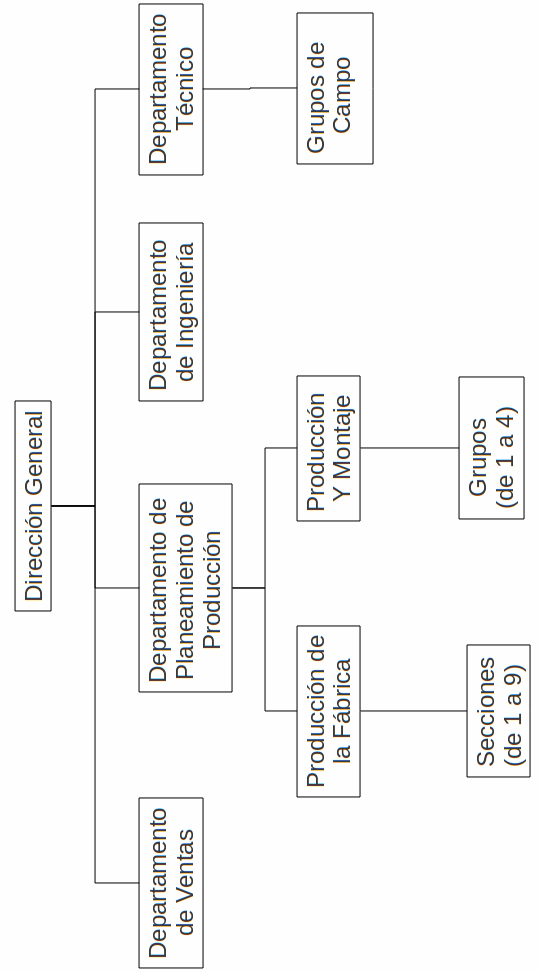
\includegraphics[width=310pt]{./herculesDiag.png}
 \end{center}


%%%%%%%%%%%%%%%%%%%%%%%%%%%%%%%%%%%%%%%%%%%%%%%%%%%%%%%%%%%%%%%%%%%%%%%%%%%%%%%%%%%%%%%%%%%%%%%%%%%%%%%


\newpage
\subsection{Tejedur\'ias Dolly}
\subsubsection{Enunciado}
\textbf{1- INTRODUCCI\'ON}\\
Este ejemplo ha sido tomado de un caso real, al cual se le han practicado algunas
simplificaciones para convertirlo en un caso al que se le pueden aplicar las técnicas
de organización.\\
Tejeduría DOLLY es una empresa dedicada a la fabricación de prendas de tejido
de punto partiendo de hilados de fibras naturales, artificiales y/o sus mezclas.
Es una empresa Pyme característica de nuestro país, en la cual se ha puesto mas
voluntarismo que aplicación de métodos científicos o profesionalizados
La empresa es del tipo familiar, con conformación legal de Sociedad Anónima, en
la cual el único director, que trabaja como gerente operativo, es un profesional de
Ingeniería, y ha dirigido esta empresa en los últimos 6 años.
La empresa comercializa sus productos en el mercado local, el 90\% a través de 10
negocios propios, y un 10\% a través de distribuidores o negocios que compran
directamente en el deposito.\\
Los diez locales están distribuidos en Capital, Gran Buenos Aires, La Plata,
Córdoba, Mar del Plata y Mendoza. Los negocios tienen de dos a cuatro
empleadas, de las cuales, una de ellas, es la encargada del negocio. En total el
plantel de vendedoras es de 45 personas.\\
Hay un jefe de ventas que supervisa, la venta de los locales, la venta mayorista y
también tiene a su cargo el depósito de productos terminados.\\
La empresa cuenta con un sistema informático que interconecta los locales con la
fabrica, que por ser un sistema un tanto rígido sufre a menudo problemas que
impiden que la información sobre ventas, stock y pedidos de los clientes se
actualicen correctamente.\\
Esto genera inconvenientes en las tiendas, que pueden quedar desabastecidas o
sobrestockeadas, además de generar inconvenientes contables.\\ \\
Las ventajas competitivas de la empresa son trabajar con materia prima de calidad,
en este caso importada de una importante firma Italiana, manteniendo un contrato
de exclusividad para la región, esto otorga una diferenciación en los productos
finales.\\
La segunda ventaja es ser una fabrica de tejido de punto integrada verticalmenete
hasta llegar al consumidos, caracteristica que es poco comun
Dolly Fabrica prendas con alto contenido de diseño con lo que ha logrado
imponerse en un mercado difícil. Nuestro análisis se realiza a mediados del año
2000 donde lo único que podíamos asegurar es que el tan pronosticado Y2K
fueron solo amenazas.\\
Al ser prendas de diseño se realizan en cantidades chicas 500 a 2000 unidades
con excepción de algunos comoditis, que se hacen de a 5000 unidades y se
repiten producciones.\\
Deben agregar a esto que cada partida se tiñen de 4 o 5 colores diferentes
Todos los años , el diseñador y el dueño de la empresa viajan a Europa para
relevar las tendencias esteticas, en modelos y colores dado que estando en
contraestación, esto le permite definir anticipadamente la producción de cada
temporada. Esto, agregado a la relación precio-calidad, resultante de su método
de comercialización pone a la empresa entre las mas importantes del mercado
La empresa tiene un negocio donde vende mercadería de diseños esclusivos y
muy cuidada calidad orientado a boutiques de alta costura, para lo cual cada
temporada, organiza un desfile con su correspondiente organización. El resto de
los negocios venden productos con un diseño Standard de acuerdo a las
necesidades del mercado al cual va dirigido.\\
En este caso también tienen muy buena acogida, logrando vender importantes
cantidades y con un nivel de ventas que si bien tiene picos se mantienen todo el
año manteniendo la operación de los locales a pleno.\\ \\
La empresa, en vista del éxito comercial que tenía, y esperando mejorar la calidad
y la productividad, en el año 1998 compró maquinas de una nueva tecnología para
reemplazar las antiguas maquinas. Estas maquinas producen prendas con la forma
exacta que debe tener cada pieza, evitando la operación de corte y todo el
desperdicio de material que se produce al cortar con los moldes los paños de tejido
Desgraciadamente no se tomaron las precauciones de tomar personal capacitado
para el manejo de esas maquinas (o capacitar personal propio) y estas no solo no
lograban la productividad Standard sino que existían muchos desperdicios de
puesta a punto o de programas mal desarrollados. También se producían
problemas de barrado (que es una línea en el tejido debido a diferencia de tensión)
Si bien se aumento la producción total con estas maquinas, no fue en la cantidad
que se esperaba y el 70\% .del tejido era realizada por las viejas maquinas
circulares.\\
Estas máquinas además como fueron compradas con credito a 5 años producían
una erogación mensual mayor que la ganancia que se producía por su uso
La fabrica se encuentra en el gran Buenos Aires, y desarrolla sus actividades en un
edificio alquilado de 4000 m2. Compra hilado de pelo (un tipo de lana) y algodón
según la temporada, el 60\% de esta materia prima es importada de Italia. El hilado
es la principal de las materias primas, al que le corresponde un porcentaje
importante del total de las compras.\\ 
A continuación se hace un a breve descripción de la empresa y su proceso
productivo.\\ \\

\textbf{2- RELEVAMIENTO DEL PROCESO PRODUCTIVO}\\ \\
El proceso productivo está dividido en siete sectores consecutivos a través de los
cuales se va transformando la materia prima hasta obtener el producto terminado,
embalado y puesto a disposición del depósito de productos terminados. La
distribución en planta es por procesos y los sectores son:\\

\begin{enumerate}
 \item Depósito de materias primas.
 \item Tejedur\'ia: 
\begin{itemize}
 \item Enconado
 \item Tejido
 \item Lavado
\end{itemize}
 \item Corte
 \item Confecci\'on
 \item Tintorer\'ia
 \item Terminaci\'on
 \item Expedici\'on
\end{enumerate}

En algunos casos, estos procesos son llevados a cabo a través de terceros, según
su naturaleza y los planes de producción. Las empresas proveedoras de estos
servicios son llamadas ``fasones'' o ``terceros''
El proceso de ``Tintorería'' que en realidad es el teñido de las prendas se realiza
cuando corresponde, y es siempre tercerizado puesto que TEJEDURIA DOLLY no
posee instalaciones para tal fin.\\

\begin{center}\textbf{\underline{Descripción de cada proceso.}}\end{center}
\textbf{\underline{2.1- Depósito de MP.}} 
 -\\ \\
\textbf{\underline{2.2- Tejeduría:}}\\
El sector de tejeduría se compone de tres partes\\
\underline{2.2.A- Enconado:} Los conos de hilado se re-enconan en casi todos los casos con
el fin de lograr una tensión pareja y acorde a los requerimientos de cada telar. En
el mismo proceso se eliminan nudos y aglomeraciones de fibras y se le aplica
parafina sólida al hilado, para facilitar su tejido.\\
\underline{2.2.B- Tejeduría:} Este es el proceso fundamental y característico de la empresa.
Se teje en los telares según especifican las órdenes de producción y las fichas de
producto.\\
Las partidas que no continúen su proceso en el sector de lavado, se someten aquí
a un control estadístico de calidad.\\
\underline{2.2.C- Lavadero:} Mediante este proceso se lavan las piezas tejidas en una solución
acuosa de distintos agentes detergentes y humectantes. Luego se las centrifuga y
finalmente se las seca con aire caliente. La finalidad de este proceso es
fundamentalmente la de lograr una estabilidad dimensional y una eliminación de
las tensiones internas adquiridas durante el tejido.\\
Las partidas listas para continuar el proceso son sometidas aquí a un control
estadístico de calidad\\
\textbf{\underline{2.3- Corte.}}\\
Para la obtención de diversas formas a partir de piezas de forma rectangular, se
recortan los paños tejidos según las formas y dimensiones especificadas en las
planillas de producto y el encogimiento previsto durante el proceso de teñido.
Luego de cortadas, las piezas se ordenan por tipo de pieza, se atan y se identifican
claramente los bultos. Las partidas ya cortadas se estiban en las estanterías si van
a ser confeccionadas por el sector de confección y se embolsan si es que van a ser
confeccionadas por talleres de terceros. Estas bolsas se apilan en forma separada.\\
\textbf{\underline{2.4- Confección}}\\
Las distintas piezas tejidas que componen una prenda se unen aquí mediante
distintos tipos de costura. Esto se hace siguiendo las reglas de arte en la materia, y
en función de las especificaciones consignadas en las fichas de cada producto.
Para la confección interna, la persona encargada del sector determina en función
de la Ficha de Producto, que máquina corresponde utilizar para cada una de las
costuras necesarias y que secuencia se seguirá hasta confeccionar todas las
prendas de la partida. La misma encargada se ocupa de la traslación de los bultos
entre los diferentes puestos de trabajo, y de la entrega de las partidas ya
confeccionadas al sector de terminación.\\
\textbf{\underline{2.5- Tintorería}}\\
Este trabajo se terceriza, pero exige un muy prolijo conteo de expedición y
recepción.\\
Este es el momento en que se toma la decisión respecto del color de las prendas.\\
Tareas previas al teñido:\\
\underline{ - Control de colores:} Se controla que los colores recibidos desde tintorería se
correspondan con la carta de colores prevista.\\
\textbf{\underline{2.6- Terminación}}\\
Cuando las partidas están confeccionadas, la persona encargada del sector de
terminación determina la secuencia de tareas a realizar sobre la prenda a los
efectos de dejarla lista para la venta. La siguiente es la secuencia general:\\
\textbf{\underline{2.7- Expedición}}\\
En este sector se almacenan las prendas para ser enviados en el momento
oportuno\\ \\
\textbf{3- DETALLES DEL PERSONAL}\\
El sector fabril se encuentra distribuido en las secciones anteriores que
detallaremos.\\
En RECEPCIÓN DE MATERIAS PRIMAS Y OFICINA DE PRODUCCIÓN se
trabaja un turno con dos personas.\\
En TEJEDURÍA existen dos encargados que supervisan el sector de ENCONADO
con dos operarios, TEJEDURÍA tiene 18 operarios y el LAVADERO que cuenta con
4 personas. Estos sectores trabajan dos turnos entre los que se divide el personal.
El sector de CORTE tiene un encargado con cuatro personas a cargo y
CONFECCIÓN tiene un encargado, un ayudante y 18 operarias.\\
Por ultimo la encargada de TERMINACIÓN tiene 14 operarias. De este sector la
mercadería pasa a DEPOSITO que cuenta con un encargado y dos personas.
Aunque este ultimo sector depende del jefe de ventas.\\
La DIRECCIÓN DE FABRICA está a cargo de un jefe de producción y cuenta
como auxiliares con una persona de mantenimiento y un chofer.\\
Existe un sector de INGENIERÍA Y CALIDAD con un encargado y dos personas a
su cargo.\\
Un JEFE DE OPERACIONES y producto con una encargada de medidas y puesta
a punto.\\
La ADMINISTRACIÓN esta dirigida por un contador y se maneja con cuatro
personas, que también asisten al gerente.\\
El personal de fabrica eran unas 80 personas, mas el personal de los locales (50
empleados) y administrativos, de logistica y directivos agregaban 20 personas.
Tenían una antigüedad promedio de 10 años y conocían bien su oficio, pero se
resistían a los cambios tecnológicos.\\ \\
Incorporación de sector.\\
En este momento (año 2000) se dispuso incorporar un sector de calidad con el fin
de reducir el desperdicio que rondaba el 20\% (adicional a lo que se explico de los
telares computarizados. Pero esta tarea tampoco fue fácil debido a que en la
industria textil se acostumbra a tener medidas aproximadas y el personal reclutado
no tenia la experiencia en el rubro como para liderar este cambio.\\ \\
\underline{Se pide} que planteen una estructura adecuada alternativa a la presentada y las
medidas que se deben poner en practica para mejorar la situación problemática en
que se encuentra la empresa.\\

\begin{center}
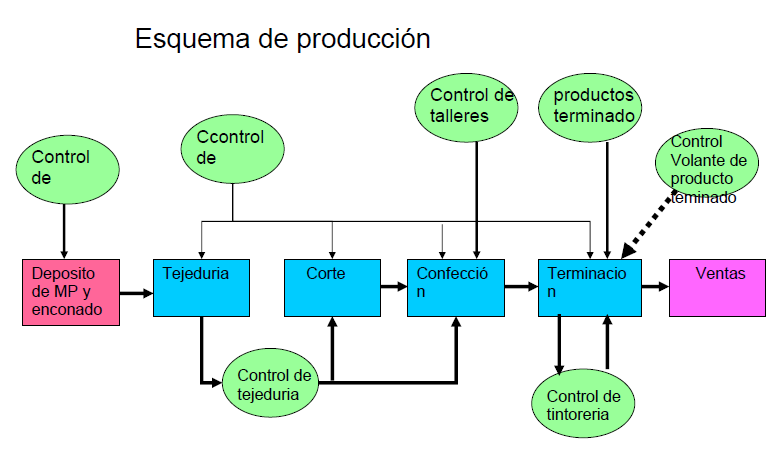
\includegraphics[scale=0.75]{./esquemaproduccionDolly.png}
\end{center}
\newpage
\subsubsection{Organigrama Derivado del Enunciado}
\begin{center} 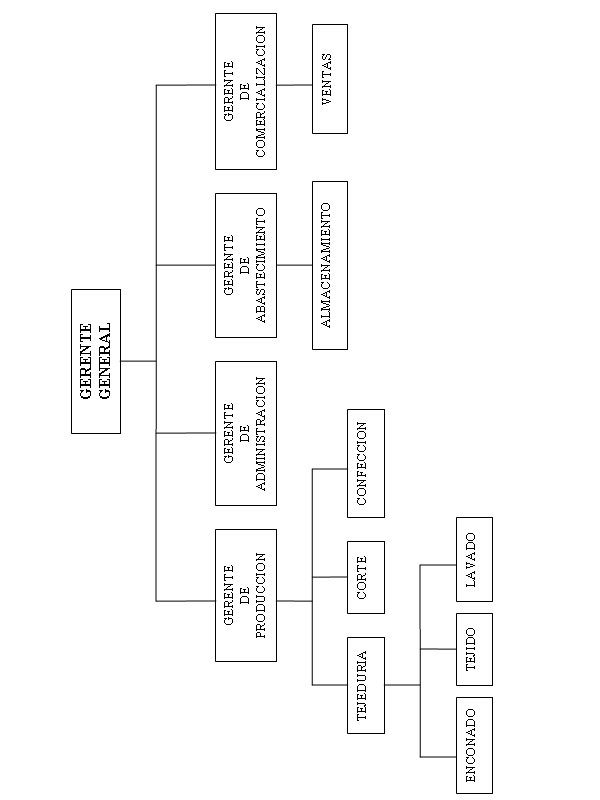
\includegraphics[scale=0.75]{./dollyDiag.png} \end{center}

\newpage
\subsubsection{Matriz FODA}
  \begin{tabular}{|c|c|}
    \hline 
      \textbf{Fortalezas} & \textbf{Oportunidades} \\ \hline
& \\
- Trabajar con materia prima de calidad. 
& - Avance tecnologico.\\
&\\
- Ser una f\'abrica de punto integrada & \\verticalmente hasta llegar al consumidor. &\\ &\\

\hline 
    \textbf{Debilidades} & \textbf{Amenazas} \\
\hline     
&\\
- Contar con un sistema inform\'atico r\'igido& - Entrada de nuevos competidores. \\que sufre continuos problemas que impide la &\\ actualizaci\'on de lainformaci\'on. &\\
&\\
- Falta de capacitaci\'on de personal para &\\el uso de las nuevas maquinarias. &\\
&\\
- Personal se resiste a cambios tecnol\'ogicos. &\\&\\ 
 \hline    
  \end{tabular}

  
\subsubsection{Medidas que se deben poner en pr\'actica}
 \begin{enumerate}
 \item Capacitar al personal para el uso de las nuevas maquinarias.
 \item Mantener actualizado el sistema inform\'atico de la empresa, de manera que la informaci\'on sobre ventas, stock y pedidos de los clientes se actualice correctamente 
y de esa forma evitar incovenientes en las tiendas e incovenientes contables.
\end{enumerate} 


%%%%%%%%%%%%%%%%%%%%%%%%%%%%%%%%%%%%%%%%%%%%%%%%%%%%%%%%%%%%%%%%%%%%%%%%%%%%%%%%%%%%%%%%%%%%%%%%%%%%%%%

\newpage
\subsection{Emporio Automotor}

\subsubsection{Enunciado}

La empresa Emporio Automotor fue fundada en 1967 como una manufacturera y distribuidora mayorista de autopartes. Inicialmente se instalaron en un garaje. Luego, 
con un espacio mayor para almacenar inventario, pudieron ofrecer una l\' inea m\' as amplia de autopartes. En esa \'epoca los automovilistas de Estados Unidos 
comenzaron a conservar sus coches por m\'as tiempo, con lo cual, en combinaci\'on con el mayor surtido de Emporio Automotor, contribuy\'o a que el negocio tuviera una 
expansi\'on explosiva hacia mediados y fines del '70. Para los primeros años de los ’90, Emporio Automotor era el mayor distribuidor independiente de autopartes de 
la regi\'on norte de Estados Unidos.\\

El año pasado la empresa se mud\'o a un nuevo conjunto de oficinas y dep\'ositos, cubriendo algo más de 30.000 metros cuadrados de superficie.\\

En la actualidad, la producci\'on se ha incrementado en un 20\% y la ocupaci\'on del depósito se ha incrementado desde el 65\% en el momento de la inauguraci\'on 
hasta alcanzar el 90\%. En el per\'iodo transcurrido, por otro lado, el volumen de ventas no ha aumentado. El r\'apido crecimiento de los inventarios indujo 
entonces a la Direcci\'on a contratar a un especialista en gesti\'on de inventarios para atacar el problema.\\

La persona adecuada para esto es Susan Torio, quien es tomada como Gerente de Abastecimiento. Sue es una Ingeniera Industrial recientemente graduada que espera con 
ansia el momento en que habr\'a de enfrentarse por primera vez con un problema del mundo real.\\

El primer d\'ia recibe un informe sobre el estado del inventario, y de las compras pendientes. Al principio de un largo listado impreso aparece una nota manuscrita de 
parte del Gerente de Compras: ''Adjunto encontrar\'a los datos referentes a los niveles de inventarios y el grado de cumplimiento con los clientes. Tenga la seguridad 
que los niveles son precisos, porque al final de la semana pasada efectuamos un conteo físico completo. Desafortunadamente, no contamos con registros compilados en 
algunas áreas, pero est\'a usted en libertad de obtenerlos por s\'i misma. ¡Bienvenida a bordo!''.\\

Un poco molesta por no tener disponible toda la información, Sue decide seleccionar al azar una pequeña muestra de aproximadamente 100 elementos, y compilar 
personalmente el inventario y el grado de cumplimiento con los clientes para formarse una idea del panorama general.\\

Los resultados de este experimento le revelan por qu\'e Emporio Automotor ha decidido convocarla. Parece que el inventario est\'a desperdigado en los lugares m\'as 
inadecuados. A pesar de que la empresa tiene unos 60 d\'ias de stock en sus inventarios, el grado de cumplimiento con los clientes no es del todo satisfactorio. \\

Sin embargo, sabe que su capacidad de introducir cambios significativos todav\'ia es limitada, a menos que sepa c\'omo generar cambios positivos de resultado 
comprobable de inmediato.\\

\newpage
\subsubsection {Interpretaci\'on}
\begin{itemize}
 \item \textbf{Resumen}\\

En principio la empresa se instal\'o como manufacturera y distribuidora mayorista de autopartes. Las demandas fueron creciendo (porque los clientes tend\'ian a tener 
sus autos cada vez por m\'as tiempo), y debieron implementarse algunos cambios para aumentar el espacio donde almacenar el inventario, de modo que se pudiera 
desarrollar una l\'inea mayor del producto. Esto deriv\'o en una r\'apida expansi\'on del negocio, y Emporio Automotor lleg\'o a convertirse en el mayor distribuidor 
independiente de autopartes de la regi\'on norte de Estados Unidos.\\

La empresa se traslad\'o a un nuevo conjunto de oficinas y dep\'ositos, que ocupaban más de 30.000 metros cuadrados de superficie.\\

En la actualidad, la producción se ha incrementado en un 20\% y la ocupaci\'on del depósito del 65\% en el momento de la inauguración alcanz\'o llegar hasta el 90\%. 
En el per\'iodo transcurrido, por otro lado, el volumen de ventas no ha aumentado.\\


\item \textbf{Problemas}\\

El r\'apido crecimiento de los inventarios indujo a la Direcci\'on a buscar un especialista en gesti\'on de inventarios para atacar el problema. Se contrat\'o entonces a 
Susan Torio como Gerente de Abastecimiento, puesto que es funcionalmente diferente al de Gerencia de Compras.\\

Torio recibe un informe sobre el estado del inventario y las compras pendientes, pero como este resulta incompleto opta por seleccionar al azar una pequeña muestra 
de alrededor de cien elementos y compilar personalmente el inventario junto con el grado de cumplimiento a los clientes. El resultado le revela que, a pesar de que la 
empresa tiene unos sesenta d\'ias de stock en sus inventarios, el último aspecto -el grado de cumplimiento con los clientes- no es del todo satisfactorio.\\

\end{itemize}
\newpage
\subsubsection{Resoluci\'on del Caso}

\begin{enumerate}
  \item Cu\'al es la estructura de la empresa antes de la contrataci\'on de Sue?\\
  - Desarrolle organigrama.
     \begin{center}
      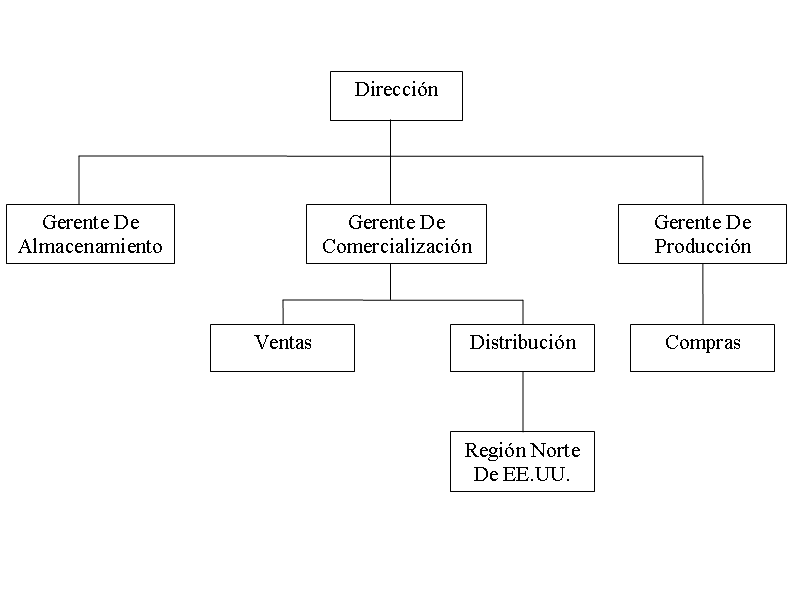
\includegraphics[scale=0.55]{./orgEmporioAutomotor.png}
     \end{center}
  
  \item Cu\'al es la diferencia funcional entre una Gerencia de Compras y Una Gerencia de Abastecimiento?
  \item P\'ongase en el lugar de Sue: C\'omo armar\'ia la estructura de la nueva Gerencia de Abastecimiento?
  \item Cuales son las Fortalezas y Debilidades de Emporio Automotor?\\ 
    \\ \textbf{Fortalezas }\\
    
    \begin{enumerate}
      \item La trayectoria de la empresa.
      \item Ser el mayor distrubuidor independiente.
      \item La infraestructura de la empresa.
     \end{enumerate}  
    \textbf{Debilidades} \\ 
   \begin{enumerate}
     \item Tener el inventario desperdigado en lugares inadecuados.
  
   \end{enumerate} 
\end{enumerate}
%%%%%%%%%%%%%%%%%%%%%%%%%%%%%%%%%%%%%%%%%%%%%%%%%%%%%%%%%%%%%%%%%%%%%%%%%%%%%%%%%%%%%%%%%%%%%%%%%%%%%%%

\newpage
\section{Imagen y Comunicaci\'on}
\subsection{Tabla de Selecci\'on de Empresas}

En la siguiente tabla aparecen las empresas que conseguimos con sus respectivos puntajes.\\
La empresa elegida es Imagen y Comunicaci\'on ya que tiene el puntaje m\'as alto y se han mostrado insteresados en ayudarnos
con el trabajo de campo.
\newcolumntype{x}[1]{%
>{\centering\hspace{0pt}}p{#1}}%
\begin{table}[h]
\begin{center}
\begin{tabular}{|c|c|c|c|x{3cm}|c|}
  \hline
  \backslashbox{Caracter\'istica}{Empresa} & Puntaje & ServiFlex & Grupo Al Sur & Imagen y Comunicaci\'on & Punto1\\
  \hline
  Contacto 		& 10 & \textit{10*} 8 & 9 & 10 & 5\\
  \hline
  Ubicaci\'on 		& 10 & \textit{10*} 8 & 8 & 8 & 8\\
  \hline
  Centralizaci\'on 	& 8  & \textit{8*} 10 & 9 & 6 & 10\\
  \hline
  Tama\~no 		& 7  & \textit{7*} 10 & 7 & 10 & 7\\
  \hline
  Disponibilidad	& 7  & \textit{7*} 6 & 4 & 9 & 7\\
  \hline
\rowcolor[gray]{0.9} Total&- & 352 & 319 & \textbf{361} & 308\\
  \hline
\end{tabular}            
\end{center}
\caption{Puntaje de Empresas}
\end{table}

\newpage

\subsection{Organigrama de la empresa}
\begin{center}
%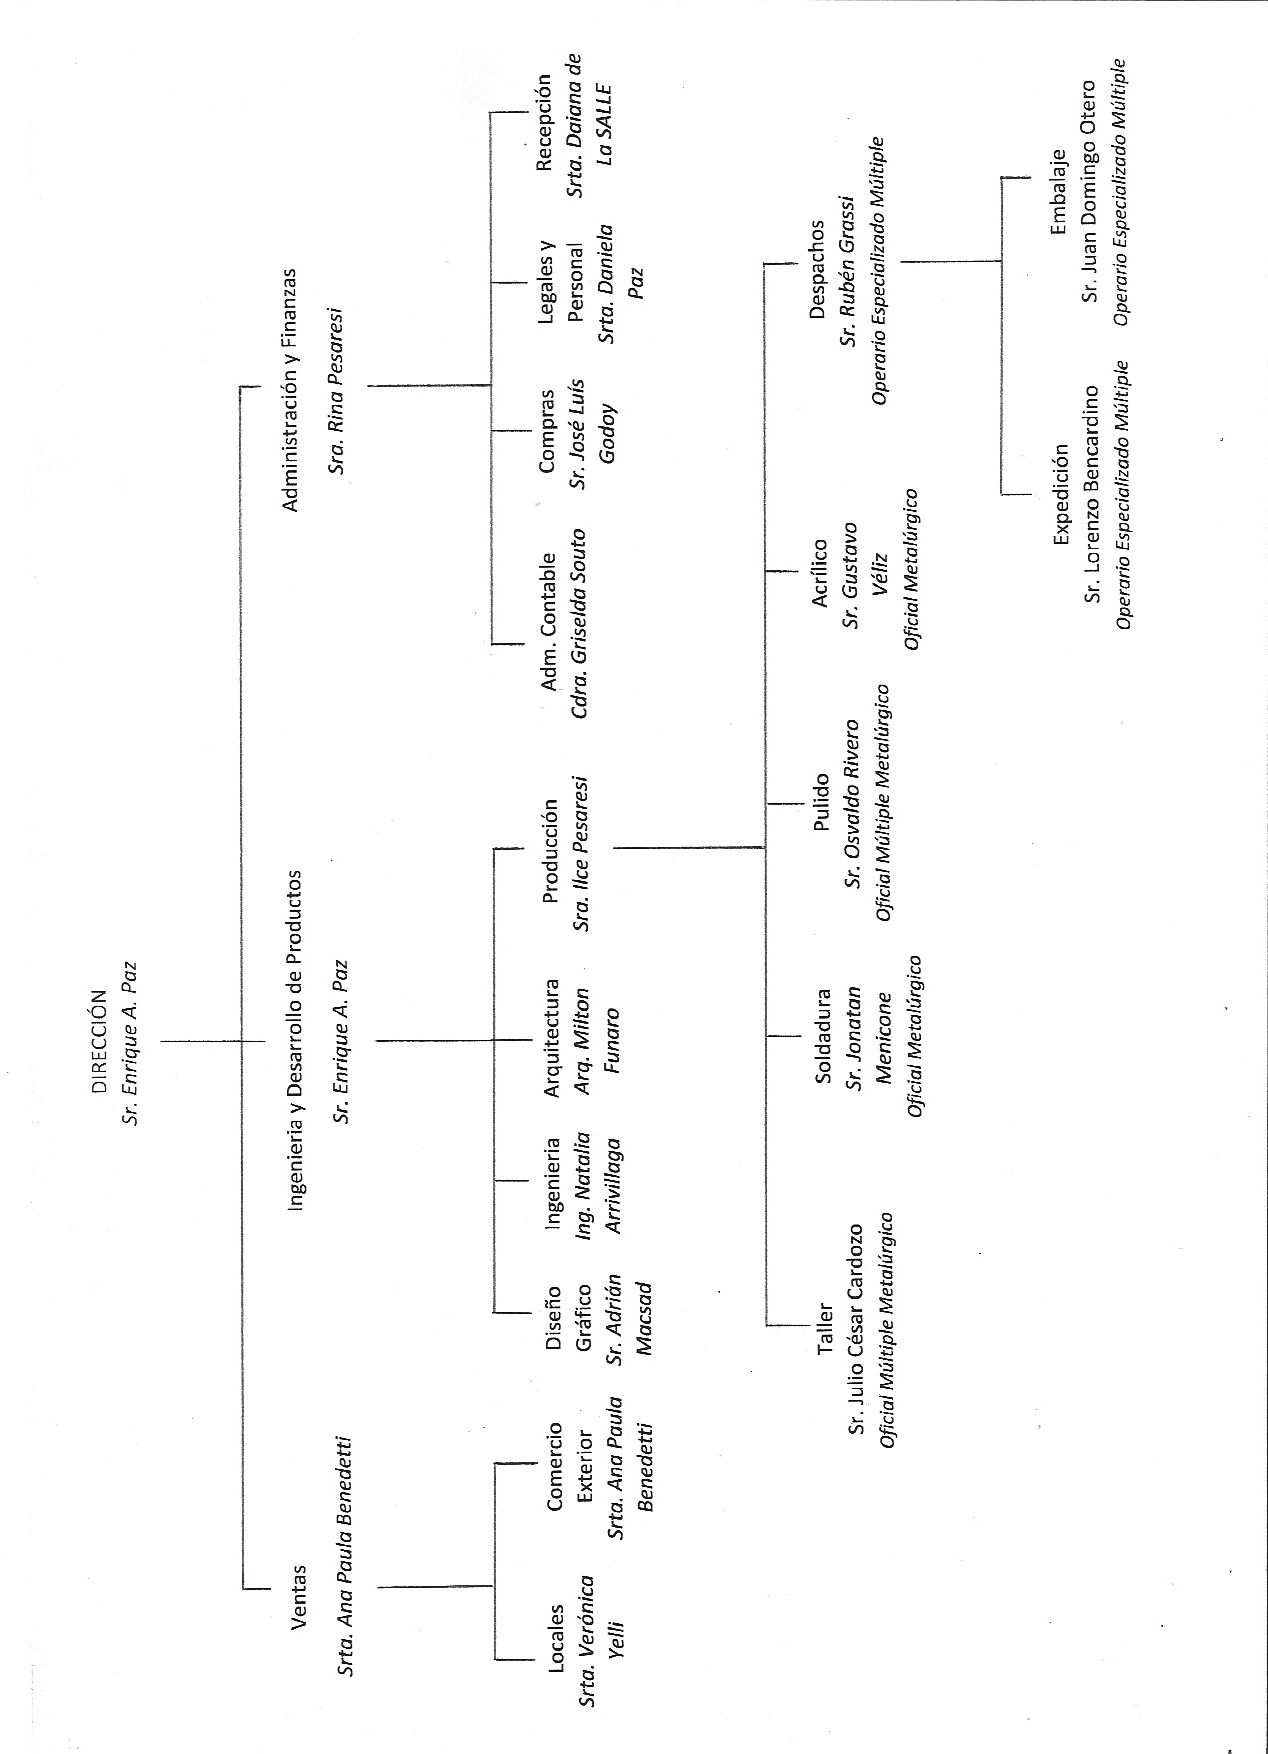
\includegraphics[width=450pt]{./imagenycomunicacion.png}
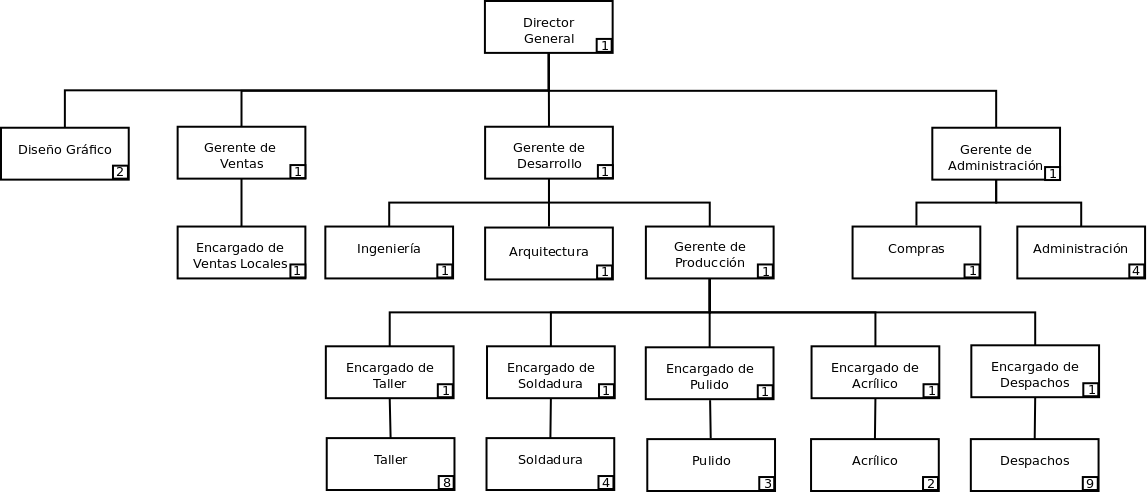
\includegraphics[scale=0.55,angle=90,keepaspectratio=true]{./organinuestro.png}
\end{center}

\newpage

\subsection{Minuta de Reuni\'on del d\'ia 4 de abril}

\begin{center}
\begin{tabular}{|c|}
	\hline
	\textbf{Fecha:} 04/04/2011    \textbf{Comienzo:} 14:00    \textbf{Fin:} 15:30 \\ \hline	

	\textbf{Lugar:} Metalurgia 'Imagen y Comunicaci\'on' S.A. \\
	\hline \textbf{Presentes:} Por parte de la empresa: Daniela Paz (Legales y Personal) \\
	Por parte de UBA: Hurtado, Pablo; Zavala, Diego; Zhang, Yi Cheng \\
	\hline \textbf{Distribuir a:} Presentes, Ing. Barmack, Daniela Paz, Grupo B1\\
	\hline
\end{tabular} 
\end{center}


\textbf{S\'intesis de los temas tratados:}

\begin{enumerate}
	\item Historia de la empresa: la creaci\'on de la empresa, una breve historia de su creaci\'on y su evoluci\'on.

	\item Organizaci\'on general de la empresa: explicaci\'on del funcionamiento de la empresa, las jerarqu\'ias en la misma, las divisiones de trabajo, y las funciones de cada gerente/jefe.

	\item Recorrido por la f\'abrica: un tour por todos los sectores de la f\'abrica para poder entender mejor su funcionamiento y c\'omo elaboran sus productos.
\end{enumerate}


\textbf{Conclusiones:} En esta primera reuni\'on, adem\'as de sus caracter\'isticas e informaci\'on general, pudimos entender bien c\'omo funciona la empresa, y la funci\'on de cada uno de los gerentes y jefes.\\


\textbf{Pasos a seguir:}\\

\begin{tabular}{|c|c|c|}
	\hline \textbf{Tarea} & \textbf{Encargado} & \textbf{Fecha de entrega} \\ 
	\hline Resumen de la entrevista & Hurtado, Pablo & 06/04/11 \\ 
	\hline Organigrama & Hurtado, Pablo & 06/04/11 \\ 
	\hline 
\end{tabular}\\\\


\textbf{Tomaron nota:} Zavala, Diego; Zhang, Yi Cheng\\
\textbf{Digitalizaci\'on:} Hurtado, Pablo; Zhang, Yi Cheng\\


\newpage


A los cuatro días del mes de abril del a\~no 2011, en la sede de Imagen y Comunicaci\'on S.A., se re\'unen los alumnos con la srta. Daniela Paz, empleada administrativa de la empresa.
Daniela trabaja all\'i hace 5 a\~nos, y si bien en el organigrama aparece como encargada de asuntos legales y de personal, tambi\'en realiza trabajos administrativos, de apoyo contable y de tesorer\'ia.

Se realiz\'o una serie de preguntas y se obtuvieron las respuestas detalladas a continuaci\'on.

\begin{itemize}

\item ¿Cu\'antos a\~nos tiene la empresa? \\
Se fund\'o en el 2000, as\'i que 11. La fecha exacta no supo decirnos.
\item ¿Cu\'al es el rubro de la misma? \\
Metal\'urgica.
\item ¿Con cu\'anto personal cuenta? \\
45 personas.
\item ¿Qu\'e operaci\'on tiene con otras empresas? \\
Tiene un contrato de exclusividad con Nike y cualquier particular que quiera poner un local que venda productos Nike 
en alguna parte de Latinoam\'erica \underline{(excepto Brasil)} tiene que ponerse en contacto con Imagen y Comunicación S.A. 
para pedir mobiliario. No tienen otros clientes. Hasta hace poco tercerizaban el trabajo de diseño gr\'afico, pero ahora lo hacen ellos mismos.
\item ¿Hace cu\'anto que es proveedor de Nike? \\
Desde que la empresa se fund\'o.
\item ¿Con cu\'antas sucursales cuenta? \\
Ninguna. Aparte de la sede, tienen un galp\'on a una cuadra, pero no hay m\'as oficinas que las de la sede.
\item ¿Cu\'al es su pol\'itica con los trabajadores? \\
La jerarqu\'a entre los trabajadores es puramente por antiguedad: los jefes de cada secci\'on son los trabajadores m\'as antiguos
 y experimentados de la misma. La comunicaci\'on es informal. No hay delegados sindicales en la empresa, aunque est\'an en la UOM.
\item ¿Existe alg\'un plan o deseo para proveer a otra empresa en el futuro? \\
S\'i existe el deseo, pero por el tamaño de la empresa ser\'ia imposible.
\item ¿Hay mucha competencia en el rubro? De ser s\'i, c\'omo la manejan? \\
En lo que hace a esta empresa en particular, no hay competencia de ning\'un tipo, dado que posee un contrato de exclusividad.
\item ¿Qu\'e productos nuevos se est\'an solicitando y deber\'an empezar a producir? (en caso de que elaboran productos a pedido de las empresas) \\
Est\'an sujetos a los cambios de l\'inea de Nike. Cuando cambia la l\'inea hay que empezar a producir muchos productos nuevos,
 para los cuales puede haber que usar t\'ecnicas diferentes a las que se ven\'ian utilizando. 
Por ejemplo, ha pasado que se ha tenido que reemplazar el sector de Acr\'ilico por un sector de Pintura por un cambio de l\'inea. 
Como los trabajadores no est\'an fuertemente especializados, se puede realizar el nuevo trabajo sin tener que hacer cambio de personal, pero con un costo de formaci\'on.
\item ¿La infraestructura (instalaciones) con la que cuentan alcanzan para el buen desarrollo del trabajo? \\
 A simple vista pareciera que no, pero si han logrado mantener un contrato de semejante exigencia durante m\'as de 11 años, debe ser suficiente.
\item ¿Cuentan con muchas tecnolog\'ias para el desarrollo de los productos o m\'as bien los productos son elaborados en forma ``artesanal''? \\
Cuentan con alta tecnolog\'ia. Tienden a renovar tecnolog\'ias en cuanto pueden (Le preguntamos si les hab\'ia pasado como en el caso Dolly; nos dijo que no, pero casi.) La figura de la cancha es la m\'aquina que corta metal con un chorro de agua con abrasivos, que tiene mayor precisi\'on que un l\'aser.
\item ¿Piensan introducir nuevas tecnolog\'ias? \\
Seguramente.
\item ¿Qui\'enes se encargan del diseño para la elaboraci\'on de los productos? Los diseños son propios o los da la empresa que pide el producto? \\
Claramente los pide Nike. Por ejemplo, una de las cosas que nos mostraron fue un escudo del Manchester Utd., y hab\'ia varios logos de Nike en las oficinas, 
y adem\'as, por la naturaleza de su trabajo (exclusivamente mobiliario de negocios deportivos), tienen que representar fielmente \'iconos que al p\'ublico le resulten 
representativos de las marcas, de modo que mucha libertad no tienen.
\item ¿Para la fabricaci\'on de sus productos, cuentan con proveedores que les venden la materia prima o se autoproveen de la misma? \\
Cuentan con proveedores. 

\end{itemize}
\newpage
\section{Presentaci\'on}
\end{document}
